\begin{figure}[H]
\centering
\caption[A priori pH Power Graph]{A priori pH power graph}
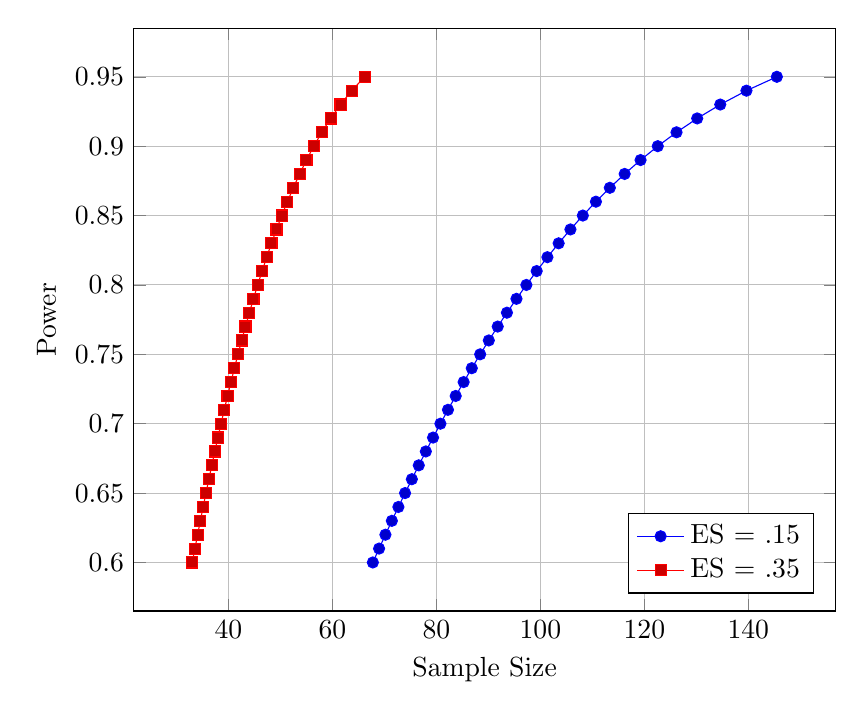
\begin{tikzpicture}
	\begin{axis}[grid=major,xlabel=Sample Size,ylabel=Power,scale=1.3, legend pos = south east]

\addplot coordinates {
(67.7774,	0.60)
(68.9775,	0.61)
(70.196,	0.62)
(71.4343,	0.63)
(72.6936	,0.64)
(73.9752,	0.65)
(75.2807,	0.66)
(76.6116,	0.67)
(77.9697,	0.68)
(79.3569,	0.69)
(80.7752,	0.70)
(82.2269,	0.71)
(83.7145,	0.72)
(85.2407,	0.73)
(86.8085	,0.74)
(88.4213,	0.75)
(90.0829	,0.76)
(91.7974,	0.77)
(93.5697	,0.78)
(95.4052,	0.79)
(97.31,	0.80)
(99.2912,	0.81)
(101.357,	0.82)
(103.517,	0.83)
(105.783,	0.84)
(108.167,	0.85)
(110.686,	0.86)
(113.36,	0.87)
(116.212,	0.88)
(119.273,	0.89)
(122.583	,0.90)
(126.19,	0.91)
(130.165	,0.92)
(134.602,	0.93)
(139.639,	0.94)
(145.49	,0.95)};
\addlegendentry{ES = .15}

\addplot coordinates{
(33.0406	,0.60)
(33.5515	,0.61)
(34.0702	,0.62)
(34.5975	,0.63)
(35.1338,	0.64)
(35.6797	,0.65)
(36.2358,	0.66)
(36.8028,	0.67)
(37.3815,	0.68)
(37.9727,	0.69)
(38.5772,	0.70)
(39.196,	0.71)
(39.8303,	0.72)
(40.481,	0.73)
(41.1496,	0.74)
(41.8375	,0.75)
(42.5462,	0.76)
(43.2777,	0.77)
(44.0338,	0.78)
(44.817,	0.79)
(45.6299,	0.80)
(46.4756,	0.81)
(47.3574,	0.82)
(48.2795,	0.83)
(49.2468,	0.84)
(50.265,	0.85)
(51.3408,	0.86)
(52.4828,	0.87)
(53.7013	,0.88)
(55.0092,	0.89)
(56.423	,0.90)
(57.9647	,0.91)
(59.6634,	0.92)
(61.5598,	0.93)
(63.7132,	0.94)
(66.2148,	0.95)};
\addlegendentry{ES = .35}

\end{axis}
\end{tikzpicture}
\label{fig:pHPowerGraph}
\end{figure}